\chapter{Introduction}
This is a grammar made as a final project for the field methods of linguistics course and Indiana University.  The course consisted of original research conducted by students, and directed by Professor Robert Botne.  The research was conducted by working with a native speaker of the Lwitaxo language in class and in private interview sessions.

\section{Lwitaxo}
The language Lwitaxo , also spelled Lwitakho and Lwidakho, is a Bantu language from South East Kenya.  Its Guthrie Bantu zone classification is JE34.  Information from Ethnologue, \url{http://www.ethnologue.com/show_language.asp?code=ida}, is shown in table \ref{tab:ethnologue} on page \pageref{tab:ethnologue} and a map of where Lwitaxo is spoken is shown in figure \ref{fig:map}.

% Table generated by Excel2LaTeX from sheet 'Sheet1'
\begin{table}[p]
  \centering
  \caption{The Ethnologue entry for the Luidakho-Luisukha-Lutirichi languages.}
\begin{tabularx}{\textwidth}{lX}
    \addlinespace
    \toprule
    {\it Population } & 306,000 (1987 BTL), increasing. Idakho 65,000, Isukha 90,000, Tiriki 100,000 (Heine and Möhlig 1980). \\
    \midrule
    {\it Region } & Western Province, Kakamega District. \\
    {\it Language map } & Kenya, reference number 26 \\
    {\it Alternate names  } & Idakho-Isukha-Tiriki \\
    {\it Dialects } & Idakho (Idaxo, Itakho), Isukha (Isuxa, Lwisukha), Tiriki. High comprehension of Logooli [rag], but resistance to each other’s pronunciation. Lexical similarity: 70\% with Logooli, 52\% with Masaba [myx] (Uganda) and Luyia [luy]. \\
    \multicolumn{ 1}{l}{{\it Classification }} & Niger-Congo, Atlantic-Congo, Volta-Congo, Benue-Congo, Bantoid, Southern, Narrow Bantu, Central, J, Masaba-Luyia (J.30), Luyia \\
    \multicolumn{ 1}{l}{{\it }} & A member of macrolanguage Oluluyia [luy] (Kenya). \\
    {\it Language use } & GIDS 5. Home, community, religious services. All Ages. Positive attitude. \\
    {\it Language development } & Literacy rate in L1: Below 1\%. Literacy rate in L2: 15\%–25\%. Taught in primary schools. Bible portions: 2000. \\
    \bottomrule
    \end{tabularx}
  \label{tab:ethnologue}
\end{table}

\begin{figure}[p] \label{fig:map}
\caption{A map of languages in Kenya.  Lwitakho is number 26, in the enlarged section.}
\centering
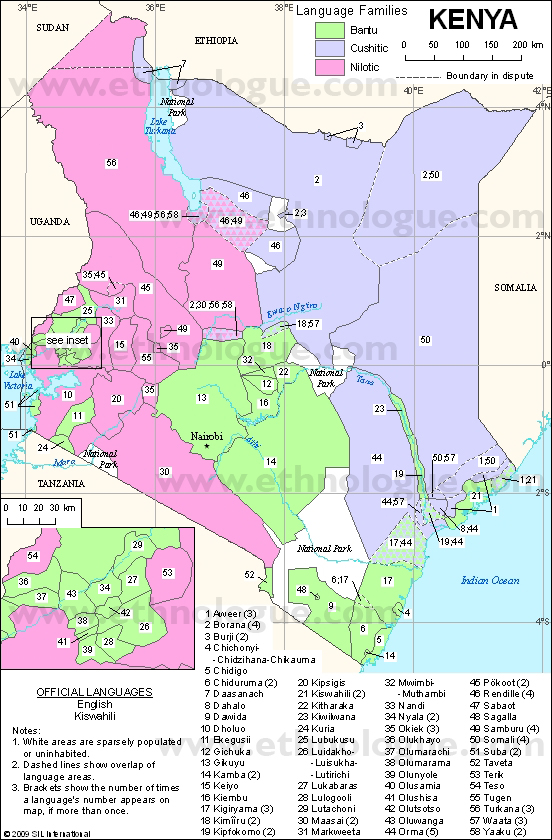
\includegraphics[width=.9\linewidth]{ken_eth}
\end{figure}

\section{Informant}
The informant for the elicitation sessions is a native speaker of Lwitaxo from Kenya.  She has lived in the United States for several years, attending graduate school, and also speaks the following languages: English, Swahili, Lubokusu, Lulokoli, Lukabarasi, and Kikuyu.